% Provenance (never printed): cycle 4 SVT, "La planete Terre, l'environnement":
% glaciers and their landforms, the cryosphere, the glaciations told; see
% sources/book1/PROVENANCE.md. Book 1, grade 8, chapter 5.
% Vocabulary guard: owns glacier; ice sheet + ice shelf + iceberg (one
% definition); sea ice; permafrost; U-shaped valley + moraine (one
% definition); ice age. "Glacial period", "interglacial" and "glacial cycle"
% belong to Book 2 g12 past-climates: here "the ice ages and the warmer times
% between them", in prose. Albedo belongs to Book 2 g10: here "reflects".
% Buoyancy and water expanding as it freezes are physics: recalled in prose.
\chapter{Ice on Earth}\label{ch:g8:ice-on-earth}

The two photographs below were taken from the same place, on a lagoon in
Alaska, 26 years apart. In 1990, a wide tongue of ice came down the \omterm{def:g1:landscapes-around-us:landform}{valley}
all the way to the water. In 2016, the ice had pulled back up the \omterm{def:g1:landscapes-around-us:landform}{valley}
and grown narrower; trees and bare \omterm{def:g3:stones-pebbles-sand:rock}{rock} filled the space it had left.
Between 1984 and 2021, satellite images show that the front of this
\omterm{def:g8:ice-on-earth:glacier}{glacier}, Pedersen \omterm{def:g8:ice-on-earth:glacier}{Glacier}, moved back about \qty{3.2}{km}.
% ledger: commons:pedersen, uw:pedersen

\begin{omfigure}
\begin{minipage}[t]{0.49\linewidth}\centering
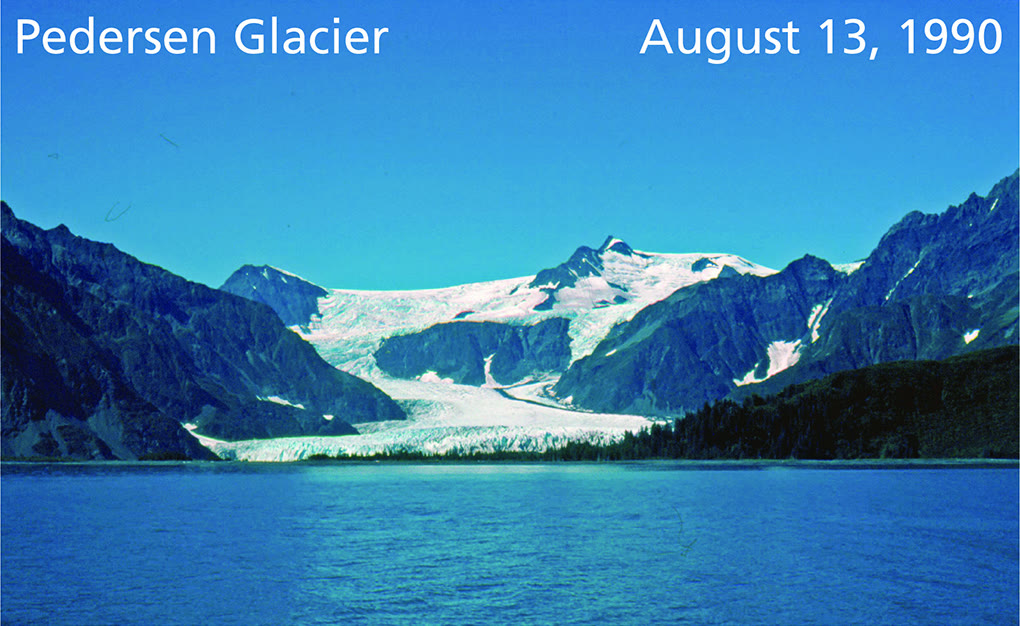
\includegraphics[width=\linewidth]{images/book1/g8-pedersen-1990.jpg}
\end{minipage}\hfill
\begin{minipage}[t]{0.49\linewidth}\centering
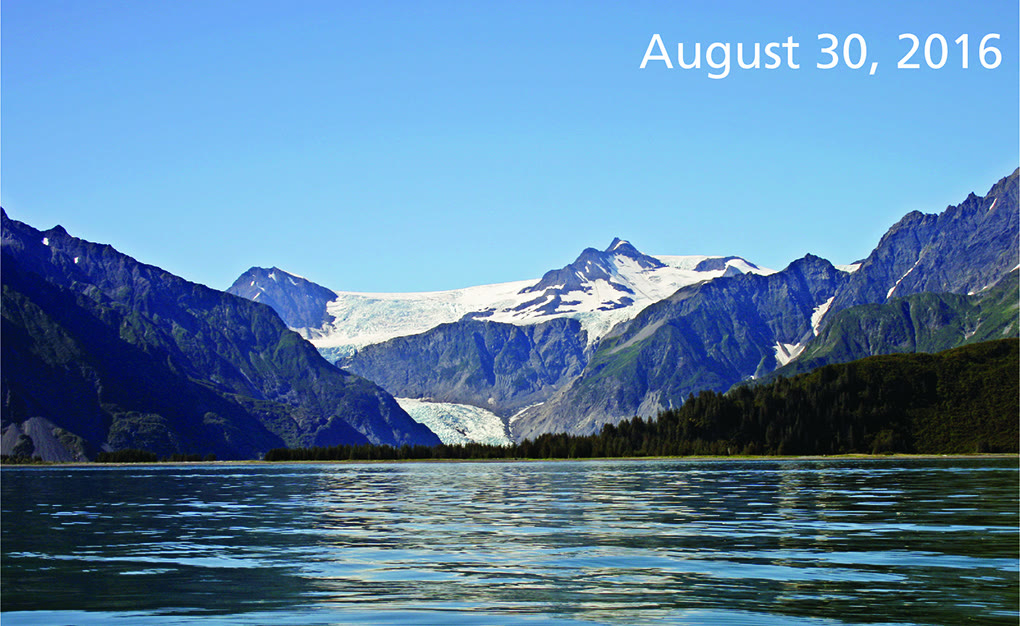
\includegraphics[width=\linewidth]{images/book1/g8-pedersen-2016.jpg}
\end{minipage}

\smallskip
{\small Pedersen \omterm{def:g8:ice-on-earth:glacier}{Glacier}, Kenai Fjords National Park, Alaska, seen from
the same place on 13~August 1990 (left, photograph by M.~Tetreau) and on
30~August 2016 (right, photograph by D.~Kurtz). U.S. National Park
Service, public domain (via Wikimedia Commons).}
% ledger: commons:pedersen
\label{fig:g8:ice-on-earth:pedersen}
\end{omfigure}

Ice covers about a tenth of the land on Earth today. It lies in \omterm{def:g1:landscapes-around-us:landform}{mountain}
\omterm{def:g1:landscapes-around-us:landform}{valleys}, in two huge sheets over Antarctica and Greenland, on the polar
\omterm{def:g2:water-on-earth:ocean}{seas} and, hidden, inside the frozen ground of the far north. This chapter
looks at each of them in turn, at how ice shapes the land, and at the
times when ice covered much more of the Earth than it does now.
% ledger: nsidc:ice-cover

\begin{recall}
\omterm{def:g4:clouds-rain-snow:precipitation}{Snow} is one kind of \omterm{def:g4:clouds-rain-snow:precipitation}{precipitation}: ice crystals that grow in a \omterm{def:g4:clouds-rain-snow:cloud}{cloud} and
fall without melting (\cref{ch:g4:clouds-rain-snow}). Running water
erodes the land, carries the pieces away and deposits them further down;
a \omterm{def:g1:landscapes-around-us:water}{river} cuts a \omterm{def:g1:landscapes-around-us:landform}{valley} (\cref{ch:g5:water-shapes-the-land}). When \omterm{def:g2:water-on-earth:ocean}{sea}
water freezes, the salt is left behind in the water around the ice
(\cref{ch:g8:the-oceans}). In physics, you learn that water expands when
it freezes, so ice is less dense than liquid water, and that a body
lighter than the water it pushes aside floats.
\end{recall}

\section{Glaciers}

High in the \omterm{def:g1:landscapes-around-us:landform}{mountains}, more \omterm{def:g4:clouds-rain-snow:precipitation}{snow} falls in winter than melts in summer.
Year after year, new \omterm{def:g4:clouds-rain-snow:precipitation}{snow} buries the old \omterm{def:g4:clouds-rain-snow:precipitation}{snow} and presses it down. The
crystals pack together, the air between them is squeezed out, and after
about a year the \omterm{def:g4:clouds-rain-snow:precipitation}{snow} has become \emph{firn}, a grainy material between
\omterm{def:g4:clouds-rain-snow:precipitation}{snow} and ice. Buried deeper and deeper, the firn turns into hard, solid
ice; for most \omterm{def:g8:ice-on-earth:glacier}{glaciers} this takes more than a hundred years.
% ledger: nsidc:firn

\begin{definition}[Glacier]\label{def:g8:ice-on-earth:glacier}
A \emph{glacier}\index{glacier} is a mass of ice, formed from \omterm{def:g4:clouds-rain-snow:precipitation}{snow} piled up over many
years, that moves slowly downhill over the land under its own weight.
\end{definition}
% ledger: nsidc:glacier-def

A \omterm{def:g8:ice-on-earth:glacier}{glacier} has two parts. In its upper part, the \emph{accumulation area},
more \omterm{def:g4:clouds-rain-snow:precipitation}{snow} falls each year than melts: the \omterm{def:g8:ice-on-earth:glacier}{glacier} gains ice. In its lower
part, the \emph{ablation area}, more ice melts each year than \omterm{def:g4:clouds-rain-snow:precipitation}{snow} falls:
the \omterm{def:g8:ice-on-earth:glacier}{glacier} loses ice. The ice gained above keeps flowing down to replace
the ice lost below. If the two balance, the front of the \omterm{def:g8:ice-on-earth:glacier}{glacier}, its
\emph{snout}, stays in the same place.
% ledger: nsidc:glacier-zones

\begin{omfigure}
\begin{tikzpicture}[font=\footnotesize, >={Stealth[length=2mm]}, xscale=1.08]
  % bedrock
  \fill[black!13] (0,4.6) -- (2,3.9) -- (4,3.0) -- (6,2.0) -- (8,1.1)
    -- (10,0.45) -- (11,0.3) -- (13,0.15) -- (13,-0.5) -- (0,-0.5) -- cycle;
  % the ice body, two zones
  \begin{scope}
    \clip (0,5.5) -- (2,4.9) -- (4,4.0) -- (6,2.9) -- (8,1.8) -- (9.4,0.95)
      -- (10,0.45) -- (8,1.1) -- (6,2.0) -- (4,3.0) -- (2,3.9) -- (0,4.6) -- cycle;
    \fill[omIce] (0,-1) rectangle (5,6);
    \fill[omSea!85] (5,-1) rectangle (11,6);
  \end{scope}
  \draw[black!60] (0,5.5) -- (2,4.9) -- (4,4.0) -- (6,2.9) -- (8,1.8)
    -- (9.4,0.95) -- (10,0.45);
  \draw[black!70, line width=0.6pt] (0,4.6) -- (2,3.9) -- (4,3.0) -- (6,2.0)
    -- (8,1.1) -- (10,0.45) -- (11,0.3) -- (13,0.15);
  % snowline
  \draw[dashed, black!70] (5,2.5) -- (5,4.15);
  \node[anchor=south] at (5,4.15) {snowfall = melting};
  % snowflakes and melting
  \foreach \x/\y in {0.5/6.1, 1.3/5.8, 2.1/5.5, 2.9/5.1, 3.7/4.8, 0.9/6.6, 1.7/6.3, 2.5/6.0, 3.3/5.6, 4.1/5.2}
    \node[omCold] at (\x,\y) {$\ast$};
  \foreach \x/\y in {6.4/2.8, 7.2/2.35, 8.0/1.9}
    \draw[omWarm, decorate, decoration={snake, amplitude=0.6mm, segment length=2mm}] (\x,\y) -- ++(0,0.6);
  % flow arrows inside the ice
  \draw[->, omDef, line width=0.9pt] (1.0,4.72) -- (2.2,4.30);
  \draw[->, omDef, line width=0.9pt] (3.0,3.95) -- (4.2,3.41);
  \draw[->, omDef, line width=0.9pt] (5.2,2.88) -- (6.4,2.28);
  \draw[->, omDef, line width=0.9pt] (7.2,1.84) -- (8.3,1.35);
  % moraine and meltwater
  \fill[omLithCongl] (10.15,0.42) .. controls (10.5,0.95) and (10.9,0.95) .. (11.2,0.29) -- cycle;
  \draw[omSea!60!black, line width=1.6pt] (10.05,0.38) .. controls (10.6,0.22) and (11.4,0.12) .. (12.9,0.08);
  % labels
  \node[align=center] at (1.9,7.15) {accumulation area:\\ snow piles up, the glacier gains ice};
  \node[align=center] at (10.0,3.3) {ablation area:\\ the ice melts, the glacier loses ice};
  \node[align=left, anchor=west, omDef] at (4.4,1.3) {the ice flows\\ downhill};
  \draw[black!60] (10.0,0.5) -- (9.6,-0.1) node[below] {snout};
  \draw[black!60] (10.7,0.85) -- (11.3,1.4) node[above] {moraine};
  \node[anchor=north east] at (12.9,0.0) {meltwater stream};
  \node at (2.2,2.6) {bedrock};
\end{tikzpicture}

{\small A \omterm{def:g1:landscapes-around-us:landform}{valley} \omterm{def:g8:ice-on-earth:glacier}{glacier} seen in a long section (a sketch, not to scale).
Above the dashed line, \omterm{def:g4:clouds-rain-snow:precipitation}{snow} piles up faster than it melts; below it, the
ice melts faster than \omterm{def:g4:clouds-rain-snow:precipitation}{snow} falls. The ice flows down from one part to the
other.}
\label{fig:g8:ice-on-earth:long-section}
\end{omfigure}

How can solid ice flow? Under the weight of the ice above it, the ice deep
in a \omterm{def:g8:ice-on-earth:glacier}{glacier} slowly deforms, the way a thick layer of cold honey spreads.
The \omterm{def:g8:ice-on-earth:glacier}{glacier} also slides over the \omterm{def:g3:stones-pebbles-sand:rock}{rock} below it, on a thin film of water or
on wet \omterm{def:g3:stones-pebbles-sand:sand}{mud}. The bottom of the \omterm{def:g8:ice-on-earth:glacier}{glacier}, rubbing on the \omterm{def:g3:stones-pebbles-sand:rock}{rock}, moves more
slowly than its top. Most \omterm{def:g8:ice-on-earth:glacier}{glaciers} move slowly and steadily; a few
suddenly \emph{surge}. In 1986, Hubbard \omterm{def:g8:ice-on-earth:glacier}{Glacier} in Alaska surged forward
about \qty{10}{m} a day, and the fastest surge on record, Kutiah \omterm{def:g8:ice-on-earth:glacier}{Glacier}
in Pakistan in 1953, averaged about \qty{112}{m} a day for three months.
% ledger: nsidc:glacier-flow, nsidc:surges

When a \omterm{def:g8:ice-on-earth:glacier}{glacier} loses more ice below than it gains above, its snout moves
back up the \omterm{def:g1:landscapes-around-us:landform}{valley}: the \omterm{def:g8:ice-on-earth:glacier}{glacier} \emph{retreats}. A retreating \omterm{def:g8:ice-on-earth:glacier}{glacier}
still flows downhill, like a conveyor belt; it just melts faster than it
flows. Muir \omterm{def:g8:ice-on-earth:glacier}{Glacier}, in Alaska, filled its whole \omterm{def:g1:landscapes-around-us:landform}{valley} down to the \omterm{def:g2:water-on-earth:ocean}{sea}
in 1941. By 2004, its snout had moved back \qty{12}{km}, and the ice
surface had come down by more than \qty{800}{m}.
% ledger: nsidc:glacier-flow, nsidc:muir

\section{How ice shapes a valley}

A \omterm{def:g8:ice-on-earth:glacier}{glacier} is a powerful tool of \omterm{def:g5:water-shapes-the-land:erosion}{erosion}. Its ice freezes onto blocks of
loose \omterm{def:g3:stones-pebbles-sand:rock}{rock} and plucks them away; the stones frozen into its base scrape
the \omterm{def:g3:stones-pebbles-sand:rock}{rock} below like sandpaper. The \omterm{def:g8:ice-on-earth:glacier}{glacier} carries all this \omterm{def:g3:stones-pebbles-sand:rock}{rock}, from
fine dust to huge boulders, down the \omterm{def:g1:landscapes-around-us:landform}{valley} like a conveyor belt, and
drops it where the ice melts.
% ledger: nps:u-valley

\begin{omfigure}
\begin{tikzpicture}[font=\footnotesize, >={Stealth[length=2mm]}]
  % V-shaped valley
  \fill[black!13] (0,3) -- (2.1,0.35) -- (2.5,0.35) -- (4.6,3) -- (4.6,-0.4) -- (0,-0.4) -- cycle;
  \draw[black!70, line width=0.6pt] (0,3) -- (2.1,0.35) -- (2.5,0.35) -- (4.6,3);
  \fill[omSea] (2.1,0.35) -- (2.5,0.35) -- (2.42,0.2) -- (2.18,0.2) -- cycle;
  \node[align=center] at (2.3,-0.85) {a river cuts a narrow\\ V-shaped valley};
  % arrow
  \draw[->, line width=1pt] (5.0,1.5) -- (6.2,1.5) node[midway, above, align=center] {a glacier\\ fills it};
  % U-shaped valley
  \begin{scope}[xshift=6.6cm]
    \fill[black!13] (0,3) .. controls (0.6,1.0) and (0.9,0.25) .. (1.6,0.2)
      -- (3.0,0.2) .. controls (3.7,0.25) and (4.0,1.0) .. (4.6,3) -- (4.6,-0.4) -- (0,-0.4) -- cycle;
    \draw[black!70, line width=0.6pt] (0,3) .. controls (0.6,1.0) and (0.9,0.25) .. (1.6,0.2)
      -- (3.0,0.2) .. controls (3.7,0.25) and (4.0,1.0) .. (4.6,3);
    \draw[dashed, black!40] (0,3) -- (2.1,0.35) -- (2.5,0.35) -- (4.6,3);
    \draw[omCold, line width=0.9pt] (0.37,2.2) -- (4.23,2.2);
    \node[omCold, anchor=south, font=\scriptsize] at (2.3,2.2) {top of the ice, long ago};
    \fill[omLithCongl] (0.75,0.95) .. controls (0.95,1.2) and (1.1,1.1) .. (1.2,0.6) -- cycle;
    \fill[omLithCongl] (3.85,0.95) .. controls (3.65,1.2) and (3.5,1.1) .. (3.4,0.6) -- cycle;
    \node[align=center] at (2.3,-0.85) {when the ice has gone: a wide\\ U-shaped valley, steep sides};
    \draw[black!60] (3.65,0.95) -- (4.85,0.6) node[right, align=left] {lateral\\ moraine};
    \node[font=\scriptsize, black!55, align=center] at (2.3,1.6) {(old V dashed)};
  \end{scope}
\end{tikzpicture}

{\small The same \omterm{def:g1:landscapes-around-us:landform}{mountain} \omterm{def:g1:landscapes-around-us:landform}{valley} in cross-section, before and after a
\omterm{def:g8:ice-on-earth:glacier}{glacier} (a sketch). The ice scours the narrow \omterm{def:g1:landscapes-around-us:water}{river} \omterm{def:g1:landscapes-around-us:landform}{valley} into a wide
trough with a broad floor and steep sides, and leaves ridges of \omterm{def:g3:stones-pebbles-sand:rock}{rock}
debris along its edges.}
\label{fig:g8:ice-on-earth:v-and-u}
\end{omfigure}

\begin{definition}[U-shaped valley and moraine]\label{def:g8:ice-on-earth:glacial-landforms}
A \emph{U-shaped valley}\index{U-shaped valley} is a \omterm{def:g1:landscapes-around-us:landform}{valley} with a broad, flat floor and steep
sides, carved by a \omterm{def:g8:ice-on-earth:glacier}{glacier} that widened and deepened a narrow V-shaped
\omterm{def:g1:landscapes-around-us:water}{river} \omterm{def:g1:landscapes-around-us:landform}{valley}. A \emph{moraine}\index{moraine} is a ridge of \omterm{def:g3:stones-pebbles-sand:rock}{rock} debris, from dust to
boulders, left by a \omterm{def:g8:ice-on-earth:glacier}{glacier}: a \emph{lateral moraine} along its side, a
\emph{terminal moraine} at its end.
\end{definition}
% ledger: usgs:erratic, nps:u-valley, nps:moraines

\omterm{def:g8:ice-on-earth:glacial-landforms}{Moraines} are useful clues. A terminal \omterm{def:g8:ice-on-earth:glacial-landforms}{moraine} far down a \omterm{def:g1:landscapes-around-us:landform}{valley}, with no
ice anywhere near it, shows how far the \omterm{def:g8:ice-on-earth:glacier}{glacier} once reached; a lateral
\omterm{def:g8:ice-on-earth:glacial-landforms}{moraine} high on a \omterm{def:g1:landscapes-around-us:landform}{valley} side shows how thick the ice once was. A large
boulder resting alone on a field, made of a \omterm{def:g3:stones-pebbles-sand:rock}{rock} found nowhere nearby, is
another clue: it is an \emph{erratic}, a \omterm{def:g3:stones-pebbles-sand:rock}{rock} carried far from its home by
a \omterm{def:g8:ice-on-earth:glacier}{glacier} and left behind when the ice melted. Erratics range from \omterm{def:g3:stones-pebbles-sand:pebble}{pebbles}
to blocks larger than a house.
% ledger: nps:moraines, usgs:erratic

\begin{inthefield}[Reading a valley shaped by ice]
On a walk in the \omterm{def:g1:landscapes-around-us:landform}{mountains}, or in a photograph of a \omterm{def:g1:landscapes-around-us:landform}{mountain} \omterm{def:g1:landscapes-around-us:landform}{valley}, look
at the shape of the \omterm{def:g1:landscapes-around-us:landform}{valley} in cross-section: a narrow V, or a wide U with
steep walls? Look across the \omterm{def:g1:landscapes-around-us:landform}{valley} floor for long ridges of jumbled
stones and soil running along its sides or across it: they may be
\omterm{def:g8:ice-on-earth:glacial-landforms}{moraines}. Look for big boulders that do not match the \omterm{def:g3:stones-pebbles-sand:rock}{rock} around them,
and for smooth \omterm{def:g3:stones-pebbles-sand:rock}{rock} surfaces scratched by long parallel lines. Stay on the
paths, keep away from the edges of steep slopes and from the ice itself,
and draw what you see in your notebook.
\end{inthefield}

\section{Ice sheets, ice shelves and icebergs}

The largest masses of ice on Earth are not in \omterm{def:g1:landscapes-around-us:landform}{mountain} \omterm{def:g1:landscapes-around-us:landform}{valleys}: they
cover whole lands. The Antarctic \omterm{def:g8:ice-on-earth:ice-sheet}{ice sheet} spreads over almost
\qty{14}{million~km^2} and is nearly \qty{4.9}{km} thick at its thickest.
The Greenland \omterm{def:g8:ice-on-earth:ice-sheet}{ice sheet} covers about \qty{1.7}{million~km^2}, four-fifths
of the island, and is over \qty{3}{km} thick. Together they hold more
than 99~\% of the ice on land, and more than two-thirds of all the \omterm{def:g2:water-on-earth:salt-fresh}{fresh
water} on Earth.
% ledger: nsidc:ice-sheets

\begin{definition}[Ice sheet, ice shelf and iceberg]\label{def:g8:ice-on-earth:ice-sheet}
An \emph{ice sheet}\index{ice sheet} is a mass of ice covering more than
\qty{50000}{km^2} of land, like a huge dome that spreads outwards in all
directions. Where ice flowing off the land reaches the \omterm{def:g2:water-on-earth:ocean}{sea} and goes on
floating on it, still joined to the ice behind it, it forms an \emph{ice
shelf}\index{ice shelf}. An \emph{iceberg}\index{iceberg} is a large block of ice, more than \qty{5}{m}
across, that has broken off a \omterm{def:g8:ice-on-earth:glacier}{glacier} or an ice shelf and floats in the
\omterm{def:g2:water-on-earth:ocean}{sea}.
\end{definition}
% ledger: nsidc:ice-sheets, nsidc:ice-shelves, nsidc:iceberg

\begin{omfigure}
\begin{minipage}[c]{0.5\linewidth}\centering
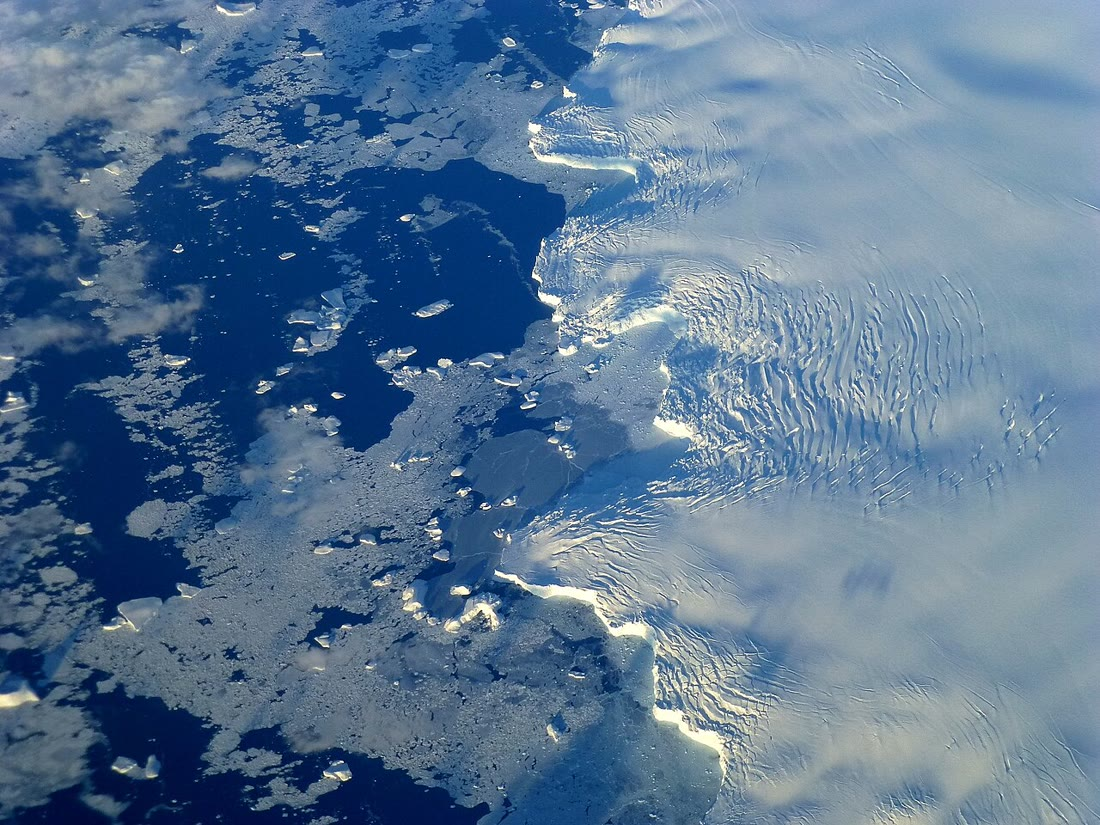
\includegraphics[width=\linewidth]{images/book1/g8-ice-shelf-edge.jpg}
\end{minipage}\hfill
\begin{minipage}[c]{0.46\linewidth}\raggedright
{\small The edge of an \omterm{def:g8:ice-on-earth:ice-sheet}{ice shelf} near Adelaide Island, off the Antarctic
Peninsula, seen from an aircraft on 28~October 2012. The thick, wrinkled
white ice on the right is the \omterm{def:g8:ice-on-earth:ice-sheet}{ice shelf}; on the left, broken pieces of
thinner \omterm{def:g8:ice-on-earth:sea-ice}{sea ice} float on the dark water. NASA, Operation IceBridge
(public domain, via Wikimedia Commons).}
\end{minipage}
% ledger: commons:ice-shelf
\label{fig:g8:ice-on-earth:ice-shelf}
\end{omfigure}

The water locked in the \omterm{def:g8:ice-on-earth:ice-sheet}{ice sheets} came from the \omterm{def:g2:water-on-earth:ocean}{ocean}: it evaporated,
fell as \omterm{def:g4:clouds-rain-snow:precipitation}{snow} and piled up on land. If all the ice of Greenland melted, the
\omterm{def:g2:water-on-earth:ocean}{sea} would rise by about \qty{7.4}{m}; if all the ice of Antarctica
melted, by about \qty{58}{m}. All the \omterm{def:g1:landscapes-around-us:landform}{mountain} \omterm{def:g8:ice-on-earth:glacier}{glaciers} of the world, more
than \num{200000} of them, would add less than half a metre.
% ledger: nsidc:ice-sheets, nsidc:ice-cover

\begin{omfigure}
\begin{tikzpicture}
\begin{axis}[omrecord, xbar, width=10.5cm, height=3.6cm, xmin=0, xmax=68,
  bar width=9pt, ytick=data, symbolic y coords={glaciers,Greenland,Antarctica},
  yticklabels={all mountain glaciers, Greenland ice sheet, Antarctic ice sheet},
  xlabel={rise of the sea if it all melted (m)}, enlarge y limits=0.3,
  nodes near coords, nodes near coords style={font=\footnotesize, anchor=west, fill=white, inner sep=1.5pt},
  ymajorgrids=false]
  \addplot[fill=omIce!80!black, draw=black!60] coordinates {(0.5,glaciers) (7.4,Greenland) (58,Antarctica)};
\end{axis}
\end{tikzpicture}

{\small How much the \omterm{def:g2:water-on-earth:ocean}{sea} would rise if each kind of land ice melted
completely (values from the National Snow and Ice Data Center; the
\omterm{def:g8:ice-on-earth:glacier}{glaciers}' value is an upper limit, ``just under half a metre'').}
% ledger: nsidc:ice-sheets, nsidc:ice-cover
\label{fig:g8:ice-on-earth:sea-level-bars}
\end{omfigure}

Floating ice is different. An \omterm{def:g8:ice-on-earth:ice-sheet}{ice shelf} or an \omterm{def:g8:ice-on-earth:ice-sheet}{iceberg} already floats on
the \omterm{def:g2:water-on-earth:ocean}{sea}: it has already pushed aside its own weight of water. When it
breaks up or melts, the \omterm{def:g2:water-on-earth:ocean}{sea} does not rise. But an \omterm{def:g8:ice-on-earth:ice-sheet}{ice shelf} holds back
the \omterm{def:g8:ice-on-earth:glacier}{glaciers} behind it, like a cork in a bottle; when the Larsen~B \omterm{def:g8:ice-on-earth:ice-sheet}{ice
shelf} in Antarctica broke apart in 2002, the \omterm{def:g8:ice-on-earth:glacier}{glaciers} behind it sped up,
some to eight times their former speed, and poured more land ice into the
\omterm{def:g2:water-on-earth:ocean}{sea}.
% ledger: nsidc:ice-shelves

\begin{inthelab}[Floating ice and ice on land]
Indoors, put a small stone in each of two clear glasses so that it sticks
out above the water when you fill them. In the first glass, float a few
ice cubes on the water. In the second, balance the same number of ice
cubes on the stone, out of the water. Fill both glasses with water to the
same level and mark it with a felt pen. Wait until all the ice has
melted, then compare the water levels with the marks. Which glass
behaves like the \omterm{def:g2:water-on-earth:ocean}{sea} when an \omterm{def:g8:ice-on-earth:ice-sheet}{iceberg} melts, and which like the \omterm{def:g2:water-on-earth:ocean}{sea} when an
\omterm{def:g8:ice-on-earth:ice-sheet}{ice sheet} melts?
\end{inthelab}

\section{Sea ice}

\omterm{def:g8:ice-on-earth:sea-ice}{Sea ice} is something else again: it is the \omterm{def:g2:water-on-earth:ocean}{sea} itself, frozen. Each
winter the surface of the polar \omterm{def:g2:water-on-earth:ocean}{oceans} freezes over a vast area; each
summer much of this ice melts again. In the Arctic, the ice is smallest
at the end of the summer, in September, and largest at the end of the
winter, in March. Satellites have measured its \emph{extent}, the area of
\omterm{def:g2:water-on-earth:ocean}{sea} where at least 15~\% of the surface is covered with ice, every day
since the late 1970s.
% ledger: nsidc:sea-ice-def

\begin{definition}[Sea ice]\label{def:g8:ice-on-earth:sea-ice}
\emph{Sea ice}\index{sea ice} is frozen \omterm{def:g2:water-on-earth:ocean}{sea} water: it forms, grows and melts in the
\omterm{def:g2:water-on-earth:ocean}{ocean} itself. It is different from \omterm{def:g8:ice-on-earth:ice-sheet}{icebergs} and ice shelves, which float
on the \omterm{def:g2:water-on-earth:ocean}{sea} but were made of \omterm{def:g4:clouds-rain-snow:precipitation}{snow} fallen on land.
\end{definition}
% ledger: nsidc:sea-ice-def

\omterm{def:g8:ice-on-earth:sea-ice}{Sea ice} matters far beyond the \omterm{def:g3:continents-and-oceans:poles}{poles}. Open \omterm{def:g2:water-on-earth:ocean}{sea} water is dark: it reflects
only about 6~\% of the sunlight that reaches it and absorbs the rest. \omterm{def:g8:ice-on-earth:sea-ice}{Sea
ice} reflects 50 to 70~\%, and \omterm{def:g8:ice-on-earth:sea-ice}{sea ice} covered with \omterm{def:g4:clouds-rain-snow:precipitation}{snow} up to 90~\%. When
the ice melts, the dark water underneath absorbs more of the Sun's energy
and warms, which melts more ice.
% ledger: nsidc:sea-ice-reflect

\begin{omfigure}
\begin{tikzpicture}
\begin{axis}[omrecord, width=13cm, height=5.4cm, xmin=1977, xmax=2027,
  ymin=3, ymax=8.2, xtick={1980,1990,...,2020},
  x tick label style={/pgf/number format/1000 sep={}},
  xlabel={year}, ylabel={extent (million km$^2$)},
  legend style={at={(0.98,0.97)}, anchor=north east, draw=none, fill=white}]
  \addplot[omCold, mark=*, mark size=1.3pt, line width=0.6pt]
    table[x=year, y=extent_Mkm2] {figdata/out/grade-8-sea_ice-extent.dat};
  \addlegendentry{September mean extent}
  \addplot[omWarm, dashed, line width=1pt]
    table[x=year, y=extent_Mkm2] {figdata/out/grade-8-sea_ice-trend.dat};
  \addlegendentry{trend line}
  \node[font=\scriptsize, anchor=north] at (axis cs:2012,3.5) {2012};
\end{axis}
\end{tikzpicture}

{\small The extent of the Arctic \omterm{def:g8:ice-on-earth:sea-ice}{sea ice} each September, 1979--2025, and
the straight line that best follows the points. Data: NSIDC Sea Ice Index,
version~4 (F.~Fetterer and others, 2025).}
% ledger: data:b1-nsidc-sea-ice (figdata/grade-8/sea_ice.py)
\label{fig:g8:ice-on-earth:sea-ice}
\end{omfigure}

The points go up and down from one year to the next: the \omterm{def:g1:watching-the-weather:weather}{weather} of each
summer counts. But over the years they clearly come down. To see the
change through the ups and downs, scientists draw a \emph{trend line}, the
straight line that passes as close as possible to all the points.
% ledger: data:b1-nsidc-sea-ice (figdata/grade-8/sea_ice.py)

\begin{method}[Reading a trend on a graph]
\begin{enumerate}
  \item Read the axes: what is measured, in which unit, over which years.
  \item Look at the points: is there a general rise, a general fall, or
        neither, behind the ups and downs?
  \item Read the trend line at the first year and at the last year.
  \item Take the difference, and divide by the number of years (or of
        decades) between them: this is the average change per year (or
        per decade).
  \item Do not read too much into one year: a single point far from the
        line is \omterm{def:g1:watching-the-weather:weather}{weather}, the line is the trend.
\end{enumerate}
\end{method}

\begin{example}[The Arctic's September ice]
On the graph, the trend line is at about \qty{7.6}{million~km^2} in 1979
and about \qty{4.1}{million~km^2} in 2025. The change is $7.6 - 4.1 =
3.5$ million~km$^2$ in $2025 - 1979 = 46$ years, that is 4.6 decades:
$3.5 \div 4.6 \approx 0.76$. The September \omterm{def:g8:ice-on-earth:sea-ice}{sea ice} has shrunk by about
\qty{0.76}{million~km^2} per decade: in 46 years, the trend line has
lost almost half of its 1979 value. The
lowest point, \qty{3.57}{million~km^2} in 2012, sits well below the line:
that summer was an exceptional one.
\end{example}
% ledger: data:b1-nsidc-sea-ice (figdata/grade-8/sea_ice.py), nsidc:sea-ice-reflect

Measurements show that the summer \omterm{def:g8:ice-on-earth:sea-ice}{sea ice} of the Arctic has become both
smaller and thinner since the 1980s, as the Arctic has warmed.
\Cref{ch:g9:climate-past-and-present} looks at how the Earth's \omterm{def:g5:weather-and-climate:climate}{climate} is
changing, and why.
% ledger: nsidc:sea-ice-reflect

\section{Permafrost}

In the far north, the cold reaches deep into the ground. Under the
tundra of North America, Greenland and northern Asia, the soil and \omterm{def:g3:stones-pebbles-sand:rock}{rock}
stay frozen all year round, and have often been frozen for thousands of
years. Only a thin top layer, the \emph{active
layer}, thaws each summer and freezes again each winter; plants grow in
it, and water that cannot drain into the frozen ground below lies in
pools on the surface.
% ledger: nsidc:permafrost

\begin{definition}[Permafrost]\label{def:g8:ice-on-earth:permafrost}
\emph{Permafrost}\index{permafrost} is ground, soil or \omterm{def:g3:stones-pebbles-sand:rock}{rock}, that stays at or below
\qty{0}{\degreeCelsius} for at least two years in a row.
\end{definition}
% ledger: nsidc:permafrost

\omterm{def:g8:ice-on-earth:permafrost}{Permafrost} lies under about \qty{23}{million~km^2}, a quarter of the land
of the \omterm{def:g3:continents-and-oceans:equator}{northern hemisphere}, and under about 85~\% of Alaska. Frozen
ground full of ice is as hard as \omterm{def:g3:stones-pebbles-sand:rock}{rock}; when its ice melts, the ground
turns to \omterm{def:g3:stones-pebbles-sand:sand}{mud} and sinks. Roads crack, buildings tilt, and pipelines can
break: where it crosses \omterm{def:g8:ice-on-earth:permafrost}{permafrost}, the Trans-Alaska Pipeline runs above
the ground for \qty{676}{km}. Thawing \omterm{def:g8:ice-on-earth:permafrost}{permafrost} also
lets the remains of plants frozen in it for thousands of years decay, and
release carbon dioxide and methane into the air.
% ledger: nsidc:permafrost, nsidc:permafrost-thaw

\begin{omfigure}
\begin{minipage}[c]{0.5\linewidth}\centering
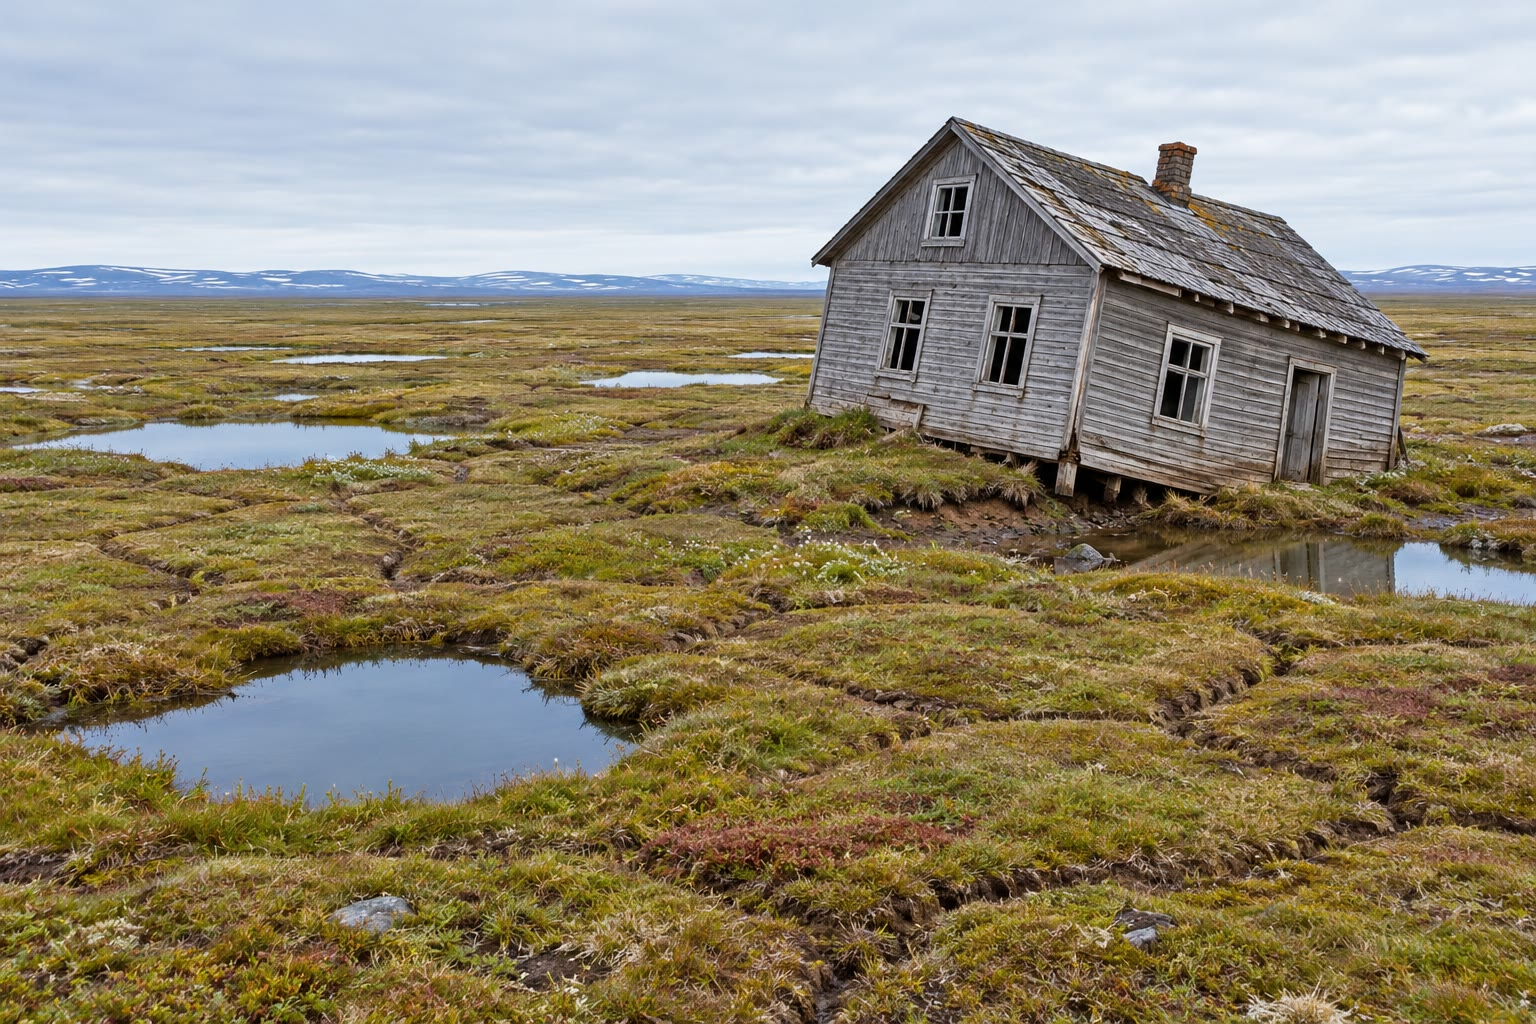
\includegraphics[width=\linewidth]{images/book1/ai/g8-permafrost-house.jpg}
\end{minipage}\hfill
\begin{minipage}[c]{0.46\linewidth}\centering
\begin{tikzpicture}[font=\footnotesize]
  \fill[omLithAlluv] (0,0) rectangle (3.2,-0.6);
  \fill[omIce!70!omLithShale] (0,-0.6) rectangle (3.2,-3.0);
  \foreach \x/\y in {0.4/-1.0, 1.5/-1.3, 2.6/-0.9, 0.9/-1.9, 2.1/-2.2, 0.5/-2.6, 2.8/-2.6}
    \fill[white] (\x,\y) ellipse (0.22 and 0.06);
  \fill[omLithShale!60] (0,-3.0) rectangle (3.2,-3.6);
  \draw[green!45!black, line width=1pt] (0,0) -- (3.2,0);
  \node[anchor=west, align=left] at (3.3,-0.3) {active layer:\\ thaws each\\ summer};
  \node[anchor=west, align=left] at (3.3,-1.8) {permafrost:\\ frozen all year,\\ lenses of ice};
  \node[anchor=west, align=left] at (3.3,-3.3) {unfrozen\\ ground};
\end{tikzpicture}
\end{minipage}

\smallskip
{\small Left: a house tilting on thawing \omterm{def:g8:ice-on-earth:permafrost}{permafrost} in the tundra
(AI-generated illustration of a generic scene). Right: the ground under
the tundra (a sketch, not to scale).}
\label{fig:g8:ice-on-earth:permafrost}
\end{omfigure}

\section{The ice ages}

Ice has not always covered the same part of the Earth. About \num{20000}
years ago, \omterm{def:g8:ice-on-earth:ice-sheet}{ice sheets} covered much of North America and of northern Europe,
including Scandinavia.
\omterm{def:g8:ice-on-earth:glacier}{Glaciers} then covered about a quarter of the land, against about a tenth
today. So much water was locked up in this ice that the \omterm{def:g2:water-on-earth:ocean}{sea} stood more
than \qty{120}{m} lower than today: parts of today's continental shelves
were dry land. From about \num{15000} years ago the \omterm{def:g8:ice-on-earth:ice-sheet}{ice sheets} melted back, and
the \omterm{def:g2:water-on-earth:ocean}{sea} rose; it reached roughly its present level about \num{8000} years
ago.
% ledger: usgs:lgm, nsidc:ice-sheets, nsidc:ice-cover

\begin{definition}[Ice age]\label{def:g8:ice-on-earth:ice-age}
An \emph{ice age}\index{ice age} is a long cold time in the Earth's history when \omterm{def:g8:ice-on-earth:ice-sheet}{ice
sheets} spread far beyond the polar regions and cover large parts of the
\omterm{def:g3:continents-and-oceans:continent}{continents}. The last ice age was at its coldest about \num{20000} years
ago and ended about \num{12000} years ago.
\end{definition}
% ledger: usgs:lgm, nps:u-valley

The clues of the last \omterm{def:g8:ice-on-earth:ice-age}{ice age} are everywhere in the lands it covered:
\omterm{def:g8:ice-on-earth:glacial-landforms}{U-shaped valleys} far from any \omterm{def:g8:ice-on-earth:glacier}{glacier} today, terminal \omterm{def:g8:ice-on-earth:glacial-landforms}{moraines} across
\omterm{def:g1:landscapes-around-us:landform}{plains}, erratic boulders lying on fields. And it was not the only one.
Over the last few hundred thousand years, the \omterm{def:g8:ice-on-earth:ice-age}{ice ages} and the warmer
times between them have followed one another again and again; we live in
one of the warm times. \Cref{ch:g9:climate-past-and-present} tells how
scientists read this long story in the ice of Antarctica itself.
% ledger: nps:u-valley, nps:moraines, usgs:erratic

\section{Exercises}

\begin{exercise}[$\star$]\label{exo:g8:ice-on-earth:1}
Using the long section of a \omterm{def:g8:ice-on-earth:glacier}{glacier} in this chapter, name: (a) the part
of the \omterm{def:g8:ice-on-earth:glacier}{glacier} where it gains ice; (b) the part where it loses ice;
(c) the front of the \omterm{def:g8:ice-on-earth:glacier}{glacier}; (d) the ridge of \omterm{def:g3:stones-pebbles-sand:rock}{rock} debris at its end.
\end{exercise}

\begin{exercise}[$\star$]\label{exo:g8:ice-on-earth:2}
% ledger: nsidc:firn, nsidc:glacier-flow, nsidc:sea-ice-def
True or false? Correct the false sentences. (a) A \omterm{def:g8:ice-on-earth:glacier}{glacier} is made of
frozen \omterm{def:g2:water-on-earth:ocean}{sea} water. (b) \omterm{def:g4:clouds-rain-snow:precipitation}{Snow} takes about a year to become firn. (c) When a
\omterm{def:g8:ice-on-earth:glacier}{glacier} retreats, its ice flows uphill. (d) \omterm{def:g8:ice-on-earth:sea-ice}{Sea ice} is smallest in the
Arctic in September.
\end{exercise}

\begin{exercise}[$\star$]\label{exo:g8:ice-on-earth:3}
% ledger: usgs:erratic, nsidc:permafrost
Give the word for each description: (a) a \omterm{def:g1:landscapes-around-us:landform}{valley} with a broad floor and
steep sides, carved by ice; (b) a boulder carried far from its home by a
\omterm{def:g8:ice-on-earth:glacier}{glacier}; (c) a floating plate of ice still joined to the ice on land;
(d) ground that stays frozen for at least two years in a row.
\end{exercise}

\begin{exercise}[$\star$]\label{exo:g8:ice-on-earth:4}
% ledger: nsidc:ice-sheets, nsidc:ice-cover
(a) Which two lands are covered by \omterm{def:g8:ice-on-earth:ice-sheet}{ice sheets} today? (b) Which of the two
would raise the \omterm{def:g2:water-on-earth:ocean}{sea} more if all its ice melted, and by how much? (c) What
share of the land on Earth is covered by ice today?
\end{exercise}

\begin{exercise}[$\star\star$]\label{exo:g8:ice-on-earth:5}
% ledger: data:b1-nsidc-sea-ice (figdata/grade-8/sea_ice.py)
Use the graph of the Arctic \omterm{def:g8:ice-on-earth:sea-ice}{sea ice} in September. (a) Read the extent in
1979 and in 2012. (b) By how many million~km$^2$ did it shrink between
these two years? (c) What fraction of the 1979 extent had gone in 2012?
Round to a simple fraction. (d) Why is it more reliable to compare the
trend line than two single years?
\end{exercise}

\begin{exercise}[$\star\star$]\label{exo:g8:ice-on-earth:6}
% ledger: nsidc:muir, uw:pedersen
Muir \omterm{def:g8:ice-on-earth:glacier}{Glacier}'s snout moved back \qty{12}{km} between 1941 and 2004.
(a) How many years is that? (b) What was its average retreat per year, in
metres? Round to the nearest ten metres. (c) Pedersen \omterm{def:g8:ice-on-earth:glacier}{Glacier} moved back
\qty{3.2}{km} between 1984 and 2021. What was its average retreat per
year? (d) Which \omterm{def:g8:ice-on-earth:glacier}{glacier} retreated faster?
\end{exercise}

\begin{exercise}[$\star\star$]\label{exo:g8:ice-on-earth:7}
Explain, in a few sentences and in order, how \omterm{def:g4:clouds-rain-snow:precipitation}{snow} falling high on a
\omterm{def:g1:landscapes-around-us:landform}{mountain} becomes the ice of a \omterm{def:g8:ice-on-earth:glacier}{glacier}'s snout, far down the \omterm{def:g1:landscapes-around-us:landform}{valley}. Use
the words \emph{firn}, \emph{accumulation area}, \emph{flows} and
\emph{ablation area}.
\end{exercise}

\begin{exercise}[$\star\star$]\label{exo:g8:ice-on-earth:8}
% ledger: nsidc:ice-shelves
Two glasses are filled to the same level. In glass A, ice cubes float on
the water; in glass B, the same ice cubes rest on a stone above the
water. (a) After the ice has melted, in which glass has the level risen?
(b) Which glass is a model of an \omterm{def:g8:ice-on-earth:ice-sheet}{iceberg} melting in the \omterm{def:g2:water-on-earth:ocean}{sea}? Of an \omterm{def:g8:ice-on-earth:ice-sheet}{ice
sheet} melting on land? (c) Why does the breaking up of an \omterm{def:g8:ice-on-earth:ice-sheet}{ice shelf}
still matter for the level of the \omterm{def:g2:water-on-earth:ocean}{sea}?
\end{exercise}

\begin{exercise}[$\star\star$]\label{exo:g8:ice-on-earth:9}
A walker crosses a wide \omterm{def:g1:landscapes-around-us:landform}{valley} with a flat floor and very steep sides. In
the middle of a field she finds a granite boulder as big as a car; all the
\omterm{def:g3:stones-pebbles-sand:rock}{rocks} of the \omterm{def:g1:landscapes-around-us:landform}{valley} are limestone. Higher up, a long ridge of jumbled
stones runs along the \omterm{def:g1:landscapes-around-us:landform}{valley} side. (a) What shape is the \omterm{def:g1:landscapes-around-us:landform}{valley}, and what
carved it? (b) How did the boulder get there? What is it called? (c) What
is the ridge, and what does its height on the \omterm{def:g1:landscapes-around-us:landform}{valley} side tell you?
\end{exercise}

\begin{exercise}[$\star\star$]\label{exo:g8:ice-on-earth:10}
% ledger: nsidc:ice-sheets
The Antarctic \omterm{def:g8:ice-on-earth:ice-sheet}{ice sheet} would raise the \omterm{def:g2:water-on-earth:ocean}{sea} by about \qty{58}{m} if it
all melted, and the Greenland \omterm{def:g8:ice-on-earth:ice-sheet}{ice sheet} by about \qty{7.4}{m}. (a) What
would a tenth of the Greenland ice add? (b) What would a hundredth of the
Antarctic ice add? (c) How many times more does Antarctica hold than
Greenland? Round to the nearest whole number.
\end{exercise}

\begin{exercise}[$\star\star\star$]\label{exo:g8:ice-on-earth:11}
% ledger: data:b1-nsidc-sea-ice (figdata/grade-8/sea_ice.py: mean_1980s, mean_2010s, trend)
The mean extent of the Arctic \omterm{def:g8:ice-on-earth:sea-ice}{sea ice} in September was
\qty{7.21}{million~km^2} over the years 1980--1989 and
\qty{4.65}{million~km^2} over the years 2010--2019. (a) One million is
$10^6$. Write both values in km$^2$, without the word ``million''.
(b) By how much did the mean extent fall between these two decades?
(c) The two decades are 30 years apart. What is the fall per decade?
Compare it with the trend line's \qty{0.76}{million~km^2} per decade.
(d) Why can a straight trend line not be extended forever into the
future?
\end{exercise}

\begin{exercise}[$\star\star\star$]\label{exo:g8:ice-on-earth:12}
% ledger: usgs:lgm (the shelf slope is exercise data)
About \num{20000} years ago the \omterm{def:g2:water-on-earth:ocean}{sea} stood about \qty{120}{m} lower than
today. Off a \omterm{def:g1:landscapes-around-us:water}{coast}, the \omterm{def:g8:the-oceans:seafloor}{continental shelf} slopes down very gently, by
\qty{1}{m} for every \qty{1}{km} out to \omterm{def:g2:water-on-earth:ocean}{sea} (exercise data). (a) How far
out to \omterm{def:g2:water-on-earth:ocean}{sea} was the \omterm{def:g1:landscapes-around-us:water}{coast} at that time? (b) Where did the water of the
missing \qty{120}{m} go? (c) Explain why a terminal \omterm{def:g8:ice-on-earth:glacial-landforms}{moraine} found today on
a \omterm{def:g1:landscapes-around-us:landform}{plain}, far from any \omterm{def:g1:landscapes-around-us:landform}{mountains}, is a clue to the same \omterm{def:g8:ice-on-earth:ice-age}{ice age}.
\end{exercise}

\section{Problem: A glacier's long retreat}

\begin{problem}[{Weekend problem --- the front of a mountain glacier has
been measured every ten years since 1960; its speed of retreat is worked
out, and the valley it leaves is read}]
\label{pb:g8:ice-on-earth:1}
% ledger: nsidc:muir, uw:pedersen, nps:moraines (figdata/grade-8/glacier_retreat.py; Glacier G and its measurements are exercise data)
Every ten years since 1960, a team has measured the position of the snout
of \omterm{def:g8:ice-on-earth:glacier}{Glacier}~G, a \omterm{def:g1:landscapes-around-us:landform}{valley} \omterm{def:g8:ice-on-earth:glacier}{glacier} in the \omterm{def:g1:landscapes-around-us:landform}{mountains}. The distance is measured
up the \omterm{def:g1:landscapes-around-us:landform}{valley} from a \omterm{def:g3:stones-pebbles-sand:rock}{rock} marker~R, painted on the \omterm{def:g1:landscapes-around-us:landform}{valley} floor at the
snout in 1960. A hut~H stands beside the \omterm{def:g1:landscapes-around-us:landform}{valley} floor, \qty{1980}{m} up
the \omterm{def:g1:landscapes-around-us:landform}{valley} from~R. The \omterm{def:g2:drawing-to-map:map}{map} shows the snout at each measurement and the
ridge just below the 1960 snout.

\begin{center}
\begin{tikzpicture}
\begin{axis}[axis equal image, width=12.5cm, xmin=-500, xmax=2600, ymin=-760, ymax=760,
  axis lines=none, clip=true]
  \fill[black!13] (axis cs:-500,-760) rectangle (axis cs:2600,760);
  \addplot[fill=white, draw=none] table[x=y, y=x] {figdata/out/grade-8-glacier_retreat-floor.dat} -- cycle;
  \addplot[fill=omIce, draw=none] table[x=y, y=x] {figdata/out/grade-8-glacier_retreat-ice.dat} -- cycle;
  \addplot[black!70, line width=0.8pt] table[x=y, y=x] {figdata/out/grade-8-glacier_retreat-walls.dat};
  \addplot[omCold, line width=0.9pt] table[x=y, y=x] {figdata/out/grade-8-glacier_retreat-fronts.dat};
  \addplot[omLithCongl!80!black, line width=3pt] table[x=y, y=x] {figdata/out/grade-8-glacier_retreat-moraine.dat};
  \addplot[only marks, mark=none, nodes near coords, point meta=explicit symbolic,
    every node near coord/.style={anchor=south, rotate=90, font=\scriptsize, inner sep=1pt}]
    table[x=y, y=x, meta=year] {figdata/out/grade-8-glacier_retreat-labels.dat};
  \addplot[only marks, mark=*, mark size=2pt] coordinates {(0,0)};
  \node[font=\footnotesize\bfseries, anchor=south east] at (axis cs:-10,10) {R};
  \addplot[only marks, mark=square*, mark size=2.6pt, omDef] coordinates {(1980,-560)};
  \node[font=\footnotesize\bfseries, anchor=north] at (axis cs:1980,-590) {H};
  \node[font=\scriptsize, anchor=west] at (axis cs:-480,-590) {up the valley $\longrightarrow$};
  \node[font=\scriptsize] at (axis cs:2250,0) {ice in 2020};
  \draw[black, line width=1.2pt] (axis cs:2000,640) -- (axis cs:2500,640)
    node[midway, below, font=\scriptsize] {\qty{500}{m}};
\end{axis}
\end{tikzpicture}

\smallskip
{\small
\begin{tabular}{|l|c|c|c|c|c|c|c|}
\hline
year & 1960 & 1970 & 1980 & 1990 & 2000 & 2010 & 2020 \\
\hline
distance of the snout from R (m) & 0 & 180 & 330 & 520 & 700 & 880 & 1080 \\
\hline
\end{tabular}}
\end{center}

\noindent\textbf{Part I --- The snout's positions.}\par\nopagebreak
\begin{enumerate}[beginpenalty=10000]
  \item How far did the snout move back between 1960 and 2020?
  \item Work out how far it moved back in each decade. In which decade
        did it move back the least? The most?
  \item Has the \omterm{def:g8:ice-on-earth:glacier}{glacier} stopped flowing downhill? Explain.
  \item The dark ridge just below the 1960 snout is made of jumbled \omterm{def:g3:stones-pebbles-sand:rock}{rock}
        debris. What is it called, and how did it form?
\end{enumerate}

\noindent\textbf{Part II --- The speed of retreat.}\par\nopagebreak
\begin{enumerate}[resume, beginpenalty=10000]
  \item What was the average retreat per decade between 1960 and 2020?
  \item And per year?
  \item Muir \omterm{def:g8:ice-on-earth:glacier}{Glacier} moved back \qty{12}{km} in 63 years, about
        \qty{190}{m} a year. How many times faster was that than
        \omterm{def:g8:ice-on-earth:glacier}{Glacier}~G?
  \item Did \omterm{def:g8:ice-on-earth:glacier}{Glacier}~G gain more ice in its accumulation area than it lost
        in its ablation area, or less? Explain.
\end{enumerate}

\noindent\textbf{Part III --- The valley it leaves.}\par\nopagebreak
\begin{enumerate}[resume, beginpenalty=10000]
  \item What shape would you expect the \omterm{def:g1:landscapes-around-us:landform}{valley} floor between R and the
        2020 snout to have in cross-section? Why?
  \item In 2020, how far was the snout from the level of the hut?
  \item At the average speed of Part~II, how many years would the snout
        need to reach the level of the hut? In which year would that be?
  \item Give one reason why this year is not a forecast.
\end{enumerate}
\end{problem}
